\chapter{Methods}
\section{Formulating our hypotheses}
\label{sec-hypothesis-reasoning}
Early attempts to integrate unsupervised state representation learning with reinforcement learning
did not yield the expected results.
One of the reasons for this was due to the fact that joint training of both algorithms 
did not work due to the instability caused by different training objectives.
Before discussing how to solve this issue, we first need to elaborate why joint training
is beneficial.
In most recent work, convolutional neural networks are used to extract features from images.
This includes reinforcement learning on images: convolutional layers precede linear layers.
The convolutional layers, with possible addition of some of the linear layers,
constitute the ``feature extraction'' portion of the policy networks
which learn from images.
In all of the related work which utilizes state representation learning and is discussed above
unsupervised learning is used train the feature extractor portion of the reinforcement learning network.
Because unsupervised learning tasks are not trained to extract states in a supervised manner (because the states
are inaccessible),
the features they learn will not exactly correspond to true states nor will they be able to
exactly learn the state transition dynamics.
This of course does not mean that approximate state representation can not be sufficiently accurate however.
For example, in \cite{stooke2021decoupling} the feature extractor trained with augmented temporal
contrast (a novel unsupervised learning task introduced in the work)
was, on some problems, able to learn features which resulted in sample-efficiency
close to training on true states.

On the other hand, by training the policy network to maximize reward, the feature extraction 
portion of the network will implicitly learn to extract features which are good enough
to choose reward-maximizing actions.
Thus, logically speaking, the feature extractor trained with just the reinforcement learning signal
has to able to extract stateful information for the images, otherwise the agent would not perform well.
However, because the reward signal is sparse and contains only indirect information about state,
the feature extractor, which contains most of the policy network parameters in simple problems,
learns slowly.

This leads us to our first hypothesis \ref{parallel-training-hypothesis}.
Assuming that the learned representations correspond to the images well,
thus also meaning that they do not destroy stateful information,
then they could be interpreted as partial extractions of states from images.
Reinforcement learning feature extraction should then learn more efficiently on top of those representations
due to fact that the search space has been constricted.
We illustrate this assumption in \ref{fig-rl-srl-features-space}.
Given the fact that neural networks have to be overparametrized in order to learn
using stochastic gradient descent and their generalization capabilities,
the feature extractors for the unsupervised learning and reinforcement learning tasks
can be the same network.
Furthermore, owing to learning properties of stochastic gradient descent,
networks need to be updated with samples taken from all available information.
In other words, they ``forget'' information they have learned unless it continues 
to be provided in subsequent gradient updates.
For this reason we suspect that continuing with unsupervised learning updates
even after the unsupervised learning loss initially diminishes
will be necessary to ensure the constriction described above.
Following this results in joint training of state representation learning
and reinforcement learning, which is why we hypothesize that it will yield higher
sample-efficiency than other training approaches.




\begin{figure}[htpb]
\begin{center}

\def\setA{(1.0,0) circle (2)}%
\def\setB{(2.7,0) circle (1.5)}%
% define the bounding box
\def\boundb{(-5,3) rectangle (9,-3)}%
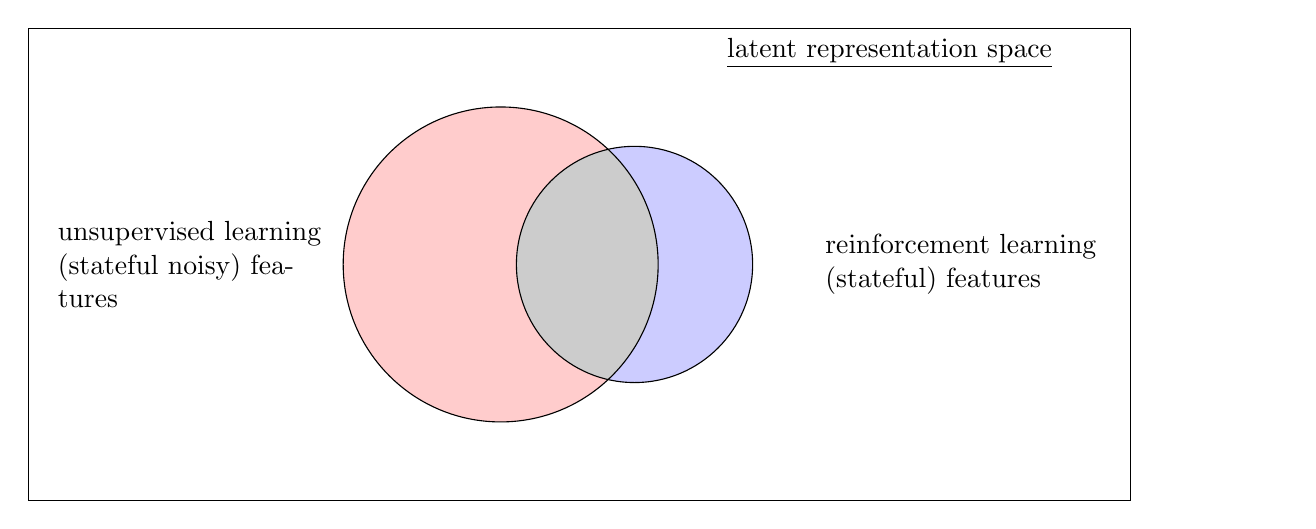
\begin{tikzpicture}
    \draw \boundb;
    % intersection
    \begin{scope}
    \clip \setA;
    \fill[black!20] \setB;
    \end{scope}
    \begin{scope}[even odd rule]% first circle without the second
    \clip \setB \boundb;
    \fill[red!20] \setA;
    \end{scope}
    \begin{scope}[even odd rule]% first circle without the second
    \clip \setA \boundb;
    \fill[blue!20] \setB;
    \end{scope}
    \draw \setA;
    \draw \setB;
    \node at (-1,0) [left, text width=3.5cm] {unsupervised learning (stateful noisy) features};
    \node at (5,0) [right, text width=3.5cm] {reinforcement learning (stateful) features};
	\node at (11,3) [below left, text width=7cm] {\underline{latent representation space}};
\end{tikzpicture}
\end{center}
\caption{Schematic of the feature extractor neural network parameter space. Since unsupervised learning
		converges much faster, it constricts the search space for the features extracted through reinforcement learning.
		This constriction is enforced joint training
of both unsupervised state representation and reinforcement learning.}
\label{fig-rl-srl-features-space}
\end{figure}

Because the objectives are different and because unsupervised learning is much faster,
we hypothesize that regularization is necessary \ref{regularization-hypothesis}.
Additionally, we hypothesize that representations which better represent true states
and state transition dynamics, i.e. the underlying Markov decision process
will better condition the reinforcement learning feature extraction task \ref{good-features-hypothesis}.

\section{Our approach}
As stated previously, the goal is to learn effective state representations
while training the policy.
We opt for a deterministic generative model to learn state representations with,
specifically a deterministic autoencoder trained with image reconstruction loss.
This is done because performance of a generative model is easier to analyse than discriminative ones.
The reinforcement learning algorithm shares its encoder with the encoder 
for state representation learning (they are the same network, with different heads attached).
Our main inspiration for this foundational approach comes from \cite{sac+ae}.
However, since we elect to work in discrete action environments, we choose \cite{rainbow}
as the underlying reinforcement learning algorithm.
Since we are not trying to achieve state-of-the-art results, we could have elected
another algorithm, but this allowed us to more easily compare our results
to those applicable in \ref{ch-related-work}, and also to have faster training times
which made experimentation easier.
We introduce changes informed by \ref{ch-related-work} in order to test our hypothesis.
Specific papers will be referenced when appropriate.
In particular this equates to the following:

\begin{enumerate}
		\item We test hypothesis \ref{parallel-training-hypothesis} with four different training modes.
		\begin{enumerate}
				\item Only the reinforcement learning algorithm is trained. This serves as 
						the control case.
				\item The autoencoder is pretrained, fixed in place, and reinforcement learning
						algorithm is trained on top of the unsupervised learning features
						without the ability to update the encoder. 
						This roughly tells us the quality of features (state representations) 
						obtained through unsupervised learning alone. \label{test-ae-fixed}
				\item Same as before, but now we update the encoder with reinforcement learning loss.
						This serves as the control case for the following mode.
				\item We jointly train the encoder both with unsupervised learning and with
						reinforcement learning loss. The encoder continues to be updated
						even after the unsupervised learning loss diminishes.
		\end{enumerate}
\item We test hypothesis \ref{good-features-hypothesis} with the following additional losses.
		\begin{enumerate}
				\item Instead of doing unsupervised learning to reconstruct the given observations,
						we also pass it action and predict the following observations.
						Since we can not pass the actions before they have been selected by the policy network,
						they are passed in the decoder (the generative part of the autoencoder).
						This thus constitutes forward prediction in pixel space.
%				\item Instead of performing forward prediction in pixel space, we now do it in latent space.
%						The autoencoder is trained with reconstructive loss as before, but we introduce
%						an additional network which predicts the latent observation. Thus this loss is calculated
%						separately and it updates the encoder along the other two losses.
%						This serves as a potentially superior version of the previous task as predictions
%						in latent space should be easier to learn that predictions in pixel space.
				\item Finally, we add inverse dynamics loss on top of the reconstruction, forward predictive 
						and reinforcement learning loss. As shown in \cite{icm}, this should encourage
						the state representation to focus the parts of the observation related to the agent
						and thus further condition state representations. As argued
						in \cite{rakelly2021mutual}, this loss alone can not be represent the MDP so it is not 
						considered in isolation.
		\end{enumerate}
\item We test hypothesis \ref{regularization-hypothesis} with the following regularization techniques.
		\begin{enumerate}
				\item Following the analysis carrier out in \cite{sac+ae}, we begin by using
						regularization techniques introduced in \cite{ghosh2019variational}.
					Since we found that joint training of state representations and reinforcement learning
					does not work without at least L2 latent space loss, we use it all joint training tests.
			\item Informed by regularization effects of denoising autoencoders, and by great success achieved
					with the random shift augmentation in \cite{drqv1, drqv2} and other recent work,
					we too use random shift augmentation on observations in unsupervised learning updates.
					This serves as our test.
		\end{enumerate}
\end{enumerate}


%We indentify the following obstacles obstructing this goal:
%\begin{enumerate}
%		\item to learn effective state representations which make the whole
%		process more efficient, the learning algorithm needs to be incentivesed
%		to embedded information relevant to the agent
%		while discarding irrelevant information
%\item as new state representations are learned, the old representations need
%		to change as little as possible so as not to compromize what
%		the policy has learned
%\end{enumerate}


%\section{Hypotheses}
%We posit the following hypotheses about features which make state representation 
%effective:
%\begin{enumerate}
%		\item representations which encode the dynamic information
%such as velocities will perform better than those which do not
%\item representations which are learned solely on observations 
%		and not both observations and the agent's actions
%		will yield worse results
%\item learning procedures which try to model only the information
%		relevant to the agent will perform even better
%\item sharing information between the policy and the state representations
%		will be benefitial
%\end{enumerate}
%
%To test whether the learning state representations helps we compare the results
%against training the policy directly on observations.
%To test the whether parallel training of the policy and the state representations
%hinders the learning process, we compare the results against the alternative training procedure
%of first learning the state representations,
%fixing them and then training the policy on these representations, i.e. the two-step training procedure.
%Finally, to test our hypotheses about the properties of state representations which yield
%higher effectiveness, we compare results of differently designed and trained state representations.
%In particular, we use an autoencoder which only reconstructs the observations given to it
%as the baseline case.
%To test whether embedding dynamic information helps, we train the same autoencoder to
%be a forward predictor. Its inputs are a number of consequtive observations and it's output 
%is the subsequent observation.
%We do this with and without also adding the agents actions as the input.
%To test whether making dynamic information more explicit helps,
%in another version we also pass the differences of each two consequtive frames.
%To test whether incentivising the state representation model to only focus on the
%dynamic information relevant to the agent helps, we train an inverse dynamics model and
%use the embeddings it generates as state representations.
%Finally, to test whether use nonlinear function approximators
%to representant policies are causing problems, we also train a tabular policy.


%In this section, we will explain the architecture of our auto-encoder and reinforcement learning algorithm. 
%This includes a description of the environment and preprocessing  
%in Section 3.0.1., 
%the collection of training data for the auto-encoder and model architecture in section 
%3.0.2. and the training of the RL agent in Section  3.0.3.


\section{Environment and Preprocessing}

We perform a comprehensive evaluation of our 
proposed method on the Arcade Learning Environment \cite{bellemare2013arcade}, 
which is composed of 57 Atari games. 
The challenge is to deploy a single algorithm and architecture, 
with a fixed set of hyper-parameters, 
to learn to play all the games given embedded latent space 
representation of the environment from auto encoder and game rewards. 
This environment is very demanding because it is both 
comprised of a large number of highly diverse games and the observations are high-dimensional.

Working with raw Atari frames, 
which are 210 x 160 pixel pictures with a 
128 color palette, is computationally expensive, therefore we do a 
basic preprocessing step to reduce the input dimensionality. 
The raw frames are down sampled to a 84 x 84 
picture and transforming their RGB representation to gray-scale.
This is standard practice in the field and it makes the training faster
without fundamentally simplifying the problem.

We constrict ourselves to games in which there is no partial observability and where
the reward is relatively dense. 
This is because we are not focusing on exploration which is necessary to solve some of the games.
Methods known to use which formulate intrinsic rewards are compatible with our approach
and can be in fact integrated with it like in \cite{exploratorysrl}.
%Cropping an 84 x 84 rectangle of the image that nearly 
%captures the playing area yields the final input representation to encoder part of the auto encoder.

\section{Module implementation}
\subsection{Tianshou}
We implement our approach as a modular extension in \cite{weng2021tianshou}.
The purpose of this choice is to make our work easily accessible and extendable.
Tianshou is an actively updated reinforcement learning library and offers the highest number reinforcement 
learning algorithms on the market.
It is based on Python and PyTorch.
It is well documented, provides tests and type hints.
It offers gym wrappers for the most popular reinforcement learning benchmarks, including
Atari.
It supports vectorization for all environments. 

The guiding principle of Tianshou is to abstract the reinforcement learning problem
as much as possible because good abstractions are the basis of modularity.
This is done by splitting reinforcement learning algorithms into the following modules:
\begin{itemize}
		\item \fbox{\texttt{Batch}}
		\item \fbox{\texttt{ReplayBuffer}}
		\item \fbox{\texttt{Policy}}
		\item \fbox{\texttt{Collector}}
		\item \fbox{\texttt{Trainer}}
\end{itemize}

These modules interact in the way depicted in \ref{tianshou-concepts}.

\begin{figure}[htpb]
		\centering
		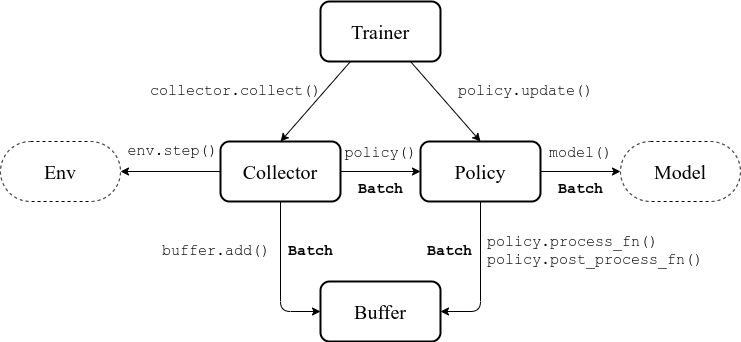
\includegraphics[width=0.8\textwidth]{"./figure/concepts_arch2.png"}
		\label{tianshou-concepts}
		\caption{Tianshou concepts}
\end{figure}


\fbox{\texttt{Batch}} is designed to store and manipulate ``hierarchical named tensors''.
Hierarchical named tensors are a set of tensors whose name forms a hierarchy.
In essence, they are nested dictionaries.

There are 7 reserved keys in \fbox{\texttt{Batch}}:
\begin{enumerate}
		\item \fbox{\texttt{obs}} --- observation at step $ t  $
		\item \fbox{\texttt{act}} --- action at step $ t  $
		\item \fbox{\texttt{rew}} --- reward at step $ t  $
		\item \fbox{\texttt{done}} --- done flag at step $ t  $
		\item \fbox{\texttt{obs\_next}} --- observation at step $ t+1  $
		\item \fbox{\texttt{info}} --- info at step $ t  $
		\item \fbox{\texttt{policy}} --- data computed by policy at step $ t  $
\end{enumerate}

\fbox{\texttt{ReplayBuffer}} stores experience data.
It's purpose is to manage \fbox{\texttt{Batch}}.
All data is stored in a circular queue.


There are different classes of policies, but all policies must inherit from \fbox{\texttt{BasePolicy}}.
Typical function are the following ones:
\begin{enumerate}
		\item \fbox{\texttt{\_\_init\_\_()}}
		\item \fbox{\texttt{forward()}} --- compute action with given observation
		\item \fbox{\texttt{process\_fn()}} --- pre-process data from the replay buffer
		\item \fbox{\texttt{learn()}} --- update policy with a given batch of data
		\item \fbox{\texttt{post\_process\_fn()}} --- pre-process data from the replay buffer
		\item \fbox{\texttt{update()}} --- this one does it all: samples from buffer,
				pre-processes data (ex. computing the n-step return),
				learn from data and post-proces sthe data (ex. update the prioritized replay buffer)
\end{enumerate}


\fbox{\texttt{Collector}}'s task is to interact with the environment
and store the observed transitions in \fbox{\texttt{ReplayBuffer}}.
\subsection{Trainer}'s task is to balance environment interactions by calling on \fbox{\texttt{Collector}}
and updating the agent by calling on \fbox{\texttt{Policy}}.


\subsection{Implementing state representation learning in Tianshou}
Surprisingly, Tianshou lacks state representation learning algorithms
which is why believe it could benefit from our work.
We implemented state representation learning as a \fbox{\texttt{Policy}}
which takes a reinforcement learning \fbox{\texttt{Policy}} as an argument.
This makes our implementation truly modular and we had to change less than 5 lines 
DQN implementation for it to work. We believe that this was due to a minor design
error in n-step return implementation, rather than our lack of foresight.
Apart from this we used Tianshou's design to our advantage.
By having the state representation learning wrapped around reinforcement learning,
we manipulate the batches sent to the reinforcement learning algorithm
and thus keep it fully encapsulated.
Data augmentation is implemented passing appropriate 
preprocessing functions to the \fbox{\texttt{Trainer}}.
The user only needs to ensure matching network dimensions to utilize 
state representation learning algorithms and pass the appropriate flag
to use the one we implemented.


\section{Network architectures}
\label{sec-net-arch}
As will be further discussed in \ref{ch-results},
an encoder just large enough to solve the reinforcement learning problem
by itself does not have the capacity to (also) solve the unsupervised pixel reconstruction
problem.
The forward prediction problem is more difficult still.
In our experiments we used 3 encoders in total, while keeping the fully connected perceptron
for reinforcement learning the same.
All decoders are simply mirror images of the corresponding encoders, where
2-dimensional convolutional layers are replaced with 2-dimensional deconvolutional layers,
and the order of the layers is flipped.

The smallest encoder is the one used in \cite{mnih2015humanlevel}.
It has only convolutional layers.
We will denote a layer's configuration as the following tuple:
(number of input channels, number of output
channels, kernel size, stride, padding).
Our smallest network is thus of the architecture:
(number of stacked frames, 32, 8, 4, 0), (32, 64, 4, 2, 0), (64, 64, 3, 1, 0).
The output of the encoder is flattened and passed to the fully connected reinforcement learning
layers. We use rectified linear units as activation functions after each layer.

In general, and for our purposes in particular, the smaller the bottleneck layer
of an autoencoder, the better it performs its job of dimensionality reduction.
For some games we were able to obtain the bottleneck of length 50, while for more visually 
complex games we used a bottleneck of length 256.
We are sure that the bottleneck layer could be made smaller with more advanced training
techniques, but this would further complicate our method and most likely 
increase the number of parameters which would negatively impact the performance of
reinforcement learning.
Furthermore, since our goal is state representation learning and not perfect reconstruction,
we believe that it is better to opt for a smaller network which compresses well enough.
Having that said, we would ideally also test the network architecture and
training procedure proposed in \cite{oh2015action}.
The architecture of the two bigger encoders differ only in the size of the bottleneck layer.
In our experiments we refer to the length of the bottleneck layer
as \textbf{features dimension}.
Their convolutional layers are the following ones. 
(number of stacked frames, 32, 3, 2, 0), 
(32, 32, 3, 2, 0),
(32, 32, 3, 2, 0),
(32, 32, 3, 2, 0).
These convolutional layers are now followed by a linear layer of the size
($32 \times 35 \times 35$, features dimension).
We use rectified linear units as activation functions after each layer but the last
which is a hyperbolic tangent function.

The both Q and V networks consist of 2 fully connected linear layers
with sizes of (features dimension, 512) and (512, number of actions $ *  $ number of atoms).

\section{Hyperparameters}
As our goal was to investigate the effectiveness of leveraging unsupervised learning
for reinforcement learning, we decided to change the underlying reinforcement learning
algorithm as little as possible.
This way we also test the effectiveness of our method as a module which is meant
to be used as an extension to the underlying algorithm.
Of course, ideally we would investigate the interplay between the two losses
to see whether particular configurations work better than others,
but we had to focus on testing our hypothesis, albeit in a somewhat limited way.
The reinforcement learning related hyperparameters can be found in \ref{table-rl-hyperparams}. \\

\begin{table}[htpb]
		\centering
		\caption{Table of reinforcement learning related hyperparameters.}
		\label{table-rl-hyperparams}
		\begin{tabular}{| c | c | }
\hline \\
\textbf{parameter} & \textbf{value} \\ \hline
epsilon test & 0.005 \\
epsilon train & 1.0 \\
epsilon train final & 0.05 \\
buffer size & 100000 \\
learning rate & 0.0001 \\
gamma & 0.99 \\
number of atoms & 51 \\
$v_{min}$ & -10.0 \\
$v_{max}$ & 10.0 \\
noisy std & 0.1 \\
alpha & 0.5 \\
beta & 0.4 \\
beta final & 1.0 \\
beta anneal steps & 5000000 \\
n-step & 3 \\
target update frequency & 500 \\
epoch & 50 \\
steps per epoch & 100000 \\
steps per collect & 10 \\
updates per step & 0.1 \\
batch size & 32 \\
number of workers for training & 10 \\
number of workers for testing & 10 \\
number of stacked frames & 4\\
				\hline
		\end{tabular}
\end{table}

Alternatively, we could have opted for hyperparameters suggested by \cite{efficientrainbow}
which are tailored for sample-efficiency.
We chose not to due to the fact that, while they are more sample-efficient,
result in longer training times.
Since we are not interested in achieving state of the art results nor
are we thoroughly experiment with reinforcement learning related hyperparameters,
we chose to perform more tests by selecting a less computationally taxing 
set of hyperparameters.

%The first step in the process is to collect data to train the auto-encoder. 
%we run a data collection module to generate the 100000 frame 
%for each stated under the result section.
%The raw images are transformed to tensors and then trained a variational autoencoder 
%with the objective of re-constructing the original image fed to the network. 
%The auto-encoder was trained for maximum  100 epochs.
%When reconstructing an image with a network bottleneck, 
%the encoder is forced to compress the original image to a smaller dimensional vector in the latent space.
%
%[By compressing the raw pixels environment to smaller dimensional 
%vector in the latent space we aim to improve the training 
%time it takes for the integrated Rl agent developed by [16] 
%and the shift in the latent space representation and its impact on 
%the RL agent learning performance.We show this in more detail in the following sections.]


%\subsection{Training the RL Agent} 
%
%In this paper we integrate auto encoder with integrated agent 
%called Rainbow[12],the selection of this architecture  was 
%based it's ability to out perform all the previous architecture.
%our main focus was to experiment with the latent space representation 
%of the environment.To address this we set up two experiment architectures one two step training and parallel training.\\
%
%\textbf{Two step Training}: First,
%we train the auto encoder with the prepossessed data and the 
%weights of the encoder are saved in file for training the agent.
%In this set up the auto encoder is not updated such that we have a static representation of the environment.
%
%second,we train the integrated agent with the results from the auto encoder.\\
%
%\textbf{Parallel Training}:
%In this set up the agent is trained using the dynamic 
%state representation from the encoder as we train both the auto 
%encoder and the integrated agent in parallel.
%This introduces stochasticity of the environment to the training  and 
%in real life control system we believe that this will set a new paradigm on the use RL.



